\begin{slideTitle}{Architecture}{Partitionnement des données}
  Découper pour mieux reigner Divide et impera
  % insérer un portrait de Nicolas Machiavel
\end{slideTitle}

\begin{slideTitle}{}{Fonctionnement}
  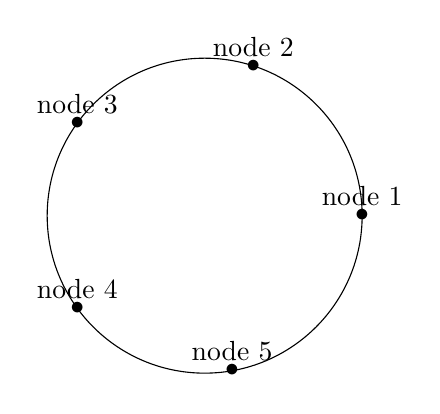
\begin{tikzpicture}
    \draw (0:2)   node[above] {node 1} node{$\bullet$};
    \draw (72:2)  node[above] {node 2} node{$\bullet$};
    \draw (144:2) node[above] {node 3} node{$\bullet$};
    \draw (216:2) node[above] {node 4} node{$\bullet$};
    \draw (280:2) node[above] {node 5} node{$\bullet$};
    \draw (0,0) circle (2) ;
  \end{tikzpicture}
\end{slideTitle}

%## Architecture
%
%Expliquer que c'est un fonctionnement P2P entre les nœuds cassandra comment
%fonctionne :
%
%- Distribution/partitionnement des données
%- Nœuds virtuels pour gérer la monté et la descente de charge
%- Réplication des données
%- Nœud coordinateur // _Ou le Quorum => et du coup le split brain, ca peut servir ^^'_
%- Niveau de consistence
